% Created 2014-05-28 Wed 12:26
\documentclass[t]{beamer}
\usepackage[utf8]{inputenc}
\usepackage[T1]{fontenc}
\usepackage{fixltx2e}
\usepackage{graphicx}
\usepackage{longtable}
\usepackage{float}
\usepackage{wrapfig}
\usepackage{soul}
\usepackage{textcomp}
\usepackage{marvosym}
\usepackage{wasysym}
\usepackage{latexsym}
\usepackage{amssymb}
\usepackage{hyperref}
\tolerance=1000
\mode<beamer>{\usetheme{TUD}}
\usepackage{tikz}
\usetikzlibrary{positioning,chains,arrows,shadows,fadings,shapes,backgrounds,snakes,matrix,patterns,plotmarks,trees,mindmap}
\usepackage{pgfpages} 
\graphicspath{{./}{figs/}{figures/}{../logos/}{../cfigures/}{../RTS-2011/figs/}{}}
\newcommand{\floor}[1]{\left\lfloor{#1}\right\rfloor}
\newcommand{\setof}[1]{\left\{{#1}\right\}}
\newcommand{\set}[2]{\left\{{#1}\mid{#2}\right\}}
\newcommand{\ceiling}[1]{\left\lceil{#1}\right\rceil}
\newcommand{\red}[1]{\textcolor{red}{#1}}
\newcommand{\blue}[1]{\textcolor{blue}{#1}}
\providecommand{\alert}[1]{\textbf{#1}}

\title{PCP in RTEMS}
\author{Kuan-Hsun Chen}

\institute{LS 12, TU Dortmund}
\date{27,07,2015}
\hypersetup{
  pdfkeywords={},
  pdfsubject={},
  pdfcreator={Emacs Org-mode version 7.9.3f}}

\tikzset{
    task/.style={shade, shading=radial, rectangle,minimum height=.1cm,
        inner color=#1!20, outer color=#1!60!gray},
    task1/.style={task=yellow, minimum width=13mm},
    task2/.style={task=green, minimum width=13mm},
    task3/.style={task=red, minimum width=13mm},
    task4/.style={task=orange, minimum width=13mm},
    task5/.style={task=blue, minimum width=13mm},
    task6/.style={task=purple, minimum width=13mm},
    task7/.style={task=cyan, minimum width=13mm},
    task8/.style={task=pink, minimum width=13mm},
}

\tikzstyle{circleNode}=[circle,thick,draw=blue!75,fill=blue!20,minimum size=6mm]
\tikzstyle{niceFill}=[thick,draw=blue!75,fill=blue!20,minimum size=6mm]

\begin{document}

\maketitle

\begin{frame}
\frametitle{Outline}

\begin{itemize}

\item Introduction of RTEMS (Pages 3-4)
\label{sec-1-1}%

\item Installation of RTEMS on Host-Computer (Pages 5-7)
\label{sec-1-2}%

\item Execute on Raspberry Pi (Pages 8-9)
\label{sec-1-3}%

\item Example of rate-monotonic multitasking (Page 10)
\label{sec-1-3}%

\item Exercises (Page 11)
\label{sec-1-4}%

\end{itemize} % ends low level
\end{frame}

\begin{frame}
\frametitle{What is RTEMS?}
\label{sec-2}
\begin{itemize}

\item Real-Time Executive for Missile Systems? \red{X}
\label{sec-2-1}%
\item The Real-Time Executive for Multiprocessor Systems (RTEMS) is an open source Real Time Operating System (RTOS) that supports open standard application programming interfaces (API) such as POSIX. 
\label{sec-2-2}%
\item It is used in space flight, medical, networking and many more embedded devices using processor 
architectures including ARM, PowerPC, Intel, Blackfin, MIPS, Microblaze and more. 
\label{sec-2-3}%
\item Commercial support is available from US and European companies, and free support comes via the active global community.
\label{sec-2-4}%
% Major decisions about RTEMS are made by the core developers in concert with the user community, guided by the Mission Statement. 
%They strive to provide regular, high quality releases, which we want to work well on a wide range of embedded targets using cross development from a variety of hosts including GNU/Linux distributions, MS Windows, BSDs, Solaris, and Mac OS. They encourage everyone to contribute changes and feedback to RTEMS.

\end{itemize} % ends low level
\end{frame}

\begin{frame}
\frametitle{Features of RTEMS}
\begin{itemize}
\item    The list of features:
\begin{itemize}

\item    multitasking capabilities
\item    homogeneous and heterogeneous multiprocessor systems
\item    \red{event-driven, priority-based, preemptive scheduling}
\item    \red{optional rate monotonic scheduling}
\item    intertask communication and synchronization
\item    \red{priority inheritance}
\item    responsive interrupt management
\item    dynamic memory allocation
\item    high level of user configurability
\end{itemize}



\item Please check:\newline \url{https://docs.rtems.org/doxygen/cpukit/html/modules.html}
\end{itemize}
\end{frame}

\begin{frame}[fragile]
\frametitle{How to install RTEMS? (1/5)}
\begin{enumerate}

\item First of all, we have to build up the cross-compiling tool chains on your host-computer.
\begin{itemize}
\item We have already prepared the environment for you to ease the complexity of installation.
\item If you want to implement on somewhere, please adopt RTEMS Source Builder \url{ftp://ftp.rtems.org/pub/rtems/people/chrisj/source-builder/source-builder.html} to aid you building packages.
\end{itemize}
\item Then, check out the repository from Github:
\begin{verbatim}
git clone https://github.com/c0066c/rtems-gpio.git
\end{verbatim}
\item Now you should have the source tree in your destination.
\end{enumerate}
\end{frame}

\begin{frame}
\frametitle{Look into the source tree (2/5)}
%  \begin{columns}
%    \column{0.6\textwidth}
%    \begin{myalterblock}{A few days into the mission.....}
%      Not long after Pathfinder started gathering meteorological data,
%      the spacecraft began experiencing total system resets, each
%      resulting in losses of data.
%    \end{myalterblock}
%    \column{1\textwidth}
%    \begin{center}
%      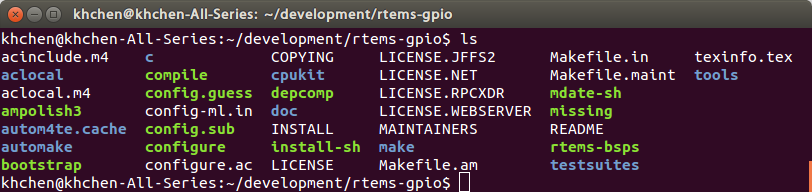
\includegraphics[width=\textwidth]{sourcetree}
%    \end{center}
%  \end{columns}
    \begin{center}
      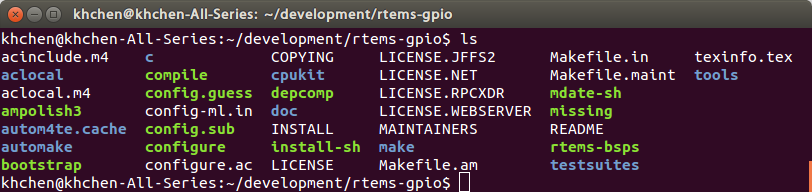
\includegraphics[width=\textwidth]{sourcetree}
    \end{center}
\begin{itemize}
\item Some important directories to us:
\begin{itemize}
\item cpukit/score/src: Provides services for all APIs (SuperCore).
\item cpukit/rtems/src: Provides RTEMS Classic APIs.
\item testsuites: Some testing programs released by RTEMS.
\item Please check the doxygen generated documentation:\newline \url{https://docs.rtems.org/doxygen/cpukit/html/modules.html}
\end{itemize}
\end{itemize}
\end{frame}

\begin{frame}
\frametitle{Hello world! (3/5)}
\begin{itemize}
\item The source code of hello world can be found in ./testsuites/samples/hello/init.c
\item Init() is similar as the main() in the standard C program.
\item In general, the init task is used to fork the multi tasks and set up the environment. Then call rtems\_task\_delete(RTEMS\_SELF) to terminate itself after initializing the system.
\item We recommend you to check the example of "Ticker" and see how to do the multitasking.
\item C User's Guide\newline \url{http://www.infres.enst.fr/~domas/astre/rtems_C_user.pdf}

\end{itemize}
\end{frame}

\begin{frame}[fragile]
\frametitle{Generating the kernel imaging (4/5)}
\begin{enumerate}
\item Under the source directory, type the command:
\begin{verbatim}
./bootstrap 
\end{verbatim}  
to run a self-sustaining process getting the configure files.
\item Trigger the configure under the building directory:
\begin{verbatim}
../rtems-gpio/configure --target=arm-rtems4.11 \
--enable-rtemsbsp=raspberrypi \
--enable-tests=samples \
--enable-posix \
--prefix=$HOME/development/rtems/4.11
\end{verbatim}   
and 
\begin{verbatim}
make install
\end{verbatim}   
\item Find up the executable file under "arm-rtems4.11/c/raspberrypi/testsuites/samples/hello"
\begin{verbatim}
make install
arm-rtems4.11-objcopy -Obinary hello.exe kernel.img
\end{verbatim}  
\end{enumerate}
\end{frame}
\begin{frame}[fragile]
\frametitle{Upload and execute the example on Raspberry Pi (5/5)}
\begin{enumerate}
\item Connect Raspberry Pi with the host computer by USBtoTTL. Please note, the pin must be connected properly, i.e., GWD, TXD, RXD, otherwise the board might be damaged.
\begin{center}
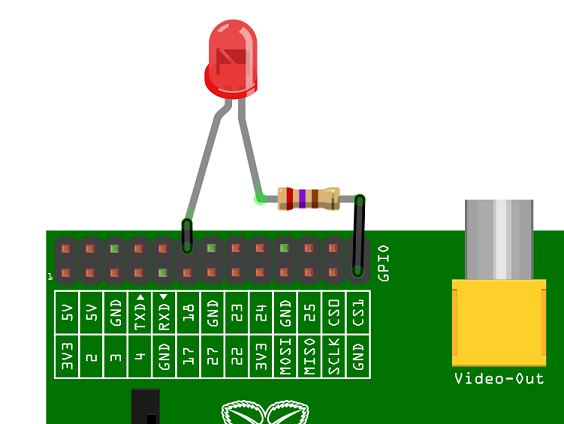
\includegraphics[width=0.3\textwidth]{gpio-led}
\end{center}
\item Copy kernel.img to "/sdcard/boot"
\item Before the power on, insert the SD-card. Please do not remove the SD-card when the power on!!
\item Open the terminal and use the following command to setup the serial debug terminal:
\begin{verbatim}
sudo screen /dev/ttyUSB0 115200
\end{verbatim}   

\end{enumerate}
\end{frame}

\begin{frame}
\frametitle{\large Rate-Monotonic Scheduling Example}

  Priority Definition: A task with a smaller period has higher
  priority, in which ties are broken arbitrarily.
  In RTEMS, the priorities of tasks need be defined when you create the tasks.

  \vskip 0.2in
  Example Schedule: $\tau_1 = (1,6,6)$, $\tau_2 = (2,8,8), \tau_3 = (4,12,12)$. [$(C_i, T_i, D_i)$]

  \begin{center}
    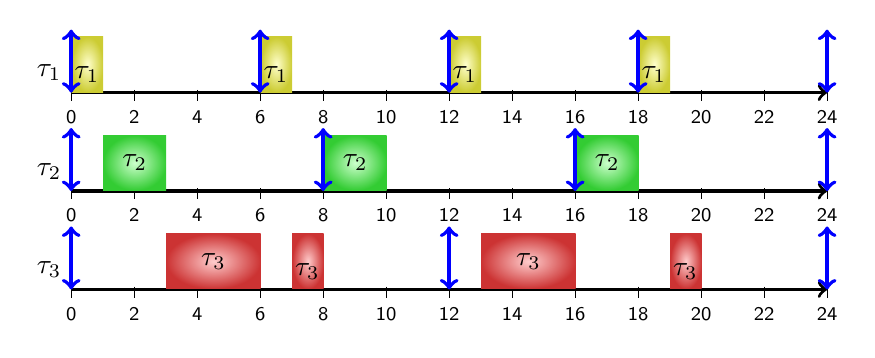
\begin{tikzpicture}[x=.4cm,font=\sffamily]
      \begin{scope}[shift={(0,2.5)}]      
      \draw[->, very thick](0,0) -- (24, 0);
      \foreach \x in {0,2,...,24}
      \draw (\x,1pt) -- (\x,-3pt) 
      node[anchor=north] {\scriptsize \x};
      \draw(0,0.25)node[anchor=east]{$\tau_1$};
      
      % \foreach \x in {0,8,16,24}
      % \draw[<-,line width=0.8mm, red](\x,0) -- (\x,1);

      \node[task1,minimum height=0.7cm, minimum width=0.4cm, anchor=south west] at (0, 0){};
      \draw(0.5,0) node[anchor=south]{ $\tau_1$};
      \node[task1,minimum height=0.7cm, minimum width=0.4cm, anchor=south west] at (6, 0){};
      \draw(6.5,0) node[anchor=south]{ $\tau_1$};
      \node[task1,minimum height=0.7cm, minimum width=0.4cm, anchor=south west] at (12, 0){};
      \draw(12.5,0) node[anchor=south]{ $\tau_1$};
      \node[task1,minimum height=0.7cm, minimum width=0.4cm, anchor=south west] at (18, 0){};
      \draw(18.5,0) node[anchor=south]{ $\tau_1$};
      \foreach \x in {0,6,12,18,24}
      \draw[<->,line width=0.5mm, blue](\x,0) -- (\x,0.8);
      \end{scope}
      \begin{scope}[shift={(0,1.25)}]      
      \draw[->, very thick](0,0) -- (24, 0);
      \foreach \x in {0,2,...,24}
      \draw (\x,1pt) -- (\x,-3pt) 
      node[anchor=north] {\scriptsize \x};
      \draw(0,0.25)node[anchor=east]{$\tau_2$};
      
      \node[task2,minimum height=0.7cm, minimum width=0.8cm, anchor=south west] at (1, 0){$\tau_2$};
      \node[task2,minimum height=0.7cm, minimum width=0.8cm, anchor=south west] at (8, 0){$\tau_2$};
      \node[task2,minimum height=0.7cm, minimum width=0.8cm, anchor=south west] at (16, 0){$\tau_2$};
      \foreach \x in {0,8,16,24}
      \draw[<->,line width=0.5mm, blue](\x,0) -- (\x,0.8);
      \end{scope}
      \draw[->, very thick](0,0) -- (24, 0);
      \foreach \x in {0,2,...,24}
      \draw (\x,1pt) -- (\x,-3pt) 
      node[anchor=north] {\scriptsize \x};
      \draw(0,0.25)node[anchor=east]{$\tau_3$};
      
      \node[task3,minimum height=0.7cm, minimum width=1.2cm, anchor=south west] at (3, 0){$\tau_3$};
      \node[task3,minimum height=0.7cm, minimum width=0.4cm, anchor=south west] at (7, 0){};
      \draw(7.5,0) node[anchor=south]{ $\tau_3$};
      \node[task3,minimum height=0.7cm, minimum width=1.2cm, anchor=south west] at (13, 0){$\tau_3$};
      \node[task3,minimum height=0.7cm, minimum width=0.4cm, anchor=south west] at (19, 0){};
      \draw(19.5,0) node[anchor=south]{ $\tau_3$};
      \foreach \x in {0,12,24}
      \draw[<->,line width=0.5mm, blue](\x,0) -- (\x,0.8);
    
     \end{tikzpicture}
  \end{center}
  
\end{frame}

\begin{frame}
\frametitle{Exercises}
\begin{enumerate}
\item Please follow the tutorial and install RTEMS on your computer. Then upload the generated kernel on Raspberry Pi to execute. Please ensure that how to compile and program the executable example.
\item Implement the Rate Monotonic example in p.10 and display the corresponding behaviours on the debug terminal.
\end{enumerate}
\end{frame}

\end{document}
